\subsection{Textual transformation with (Un)Parser}
In chapter \ref{TGG_overview_chapter} we also mentioned the possibility to transfrm between an Abstract Syntx Tree (AST) and textfiles with parser and unparser. In this chapter we will look at such a transformation. But as example we only examine the transformation from a textfile to an AST with a parser.
\newline
\newline
As like before we use the dictionary example. We will translate textfiles into our dictionary model. So first have a look at Fig.~\ref{textual_syntax}. Here you can see the textual syntax of a dictionary file. The words in capital letters are our tokens for dictionary files.
\newline
As the next step we have to generate a lexer to indicate the tokens.

\begin{figure}[htbp]
	\centering
	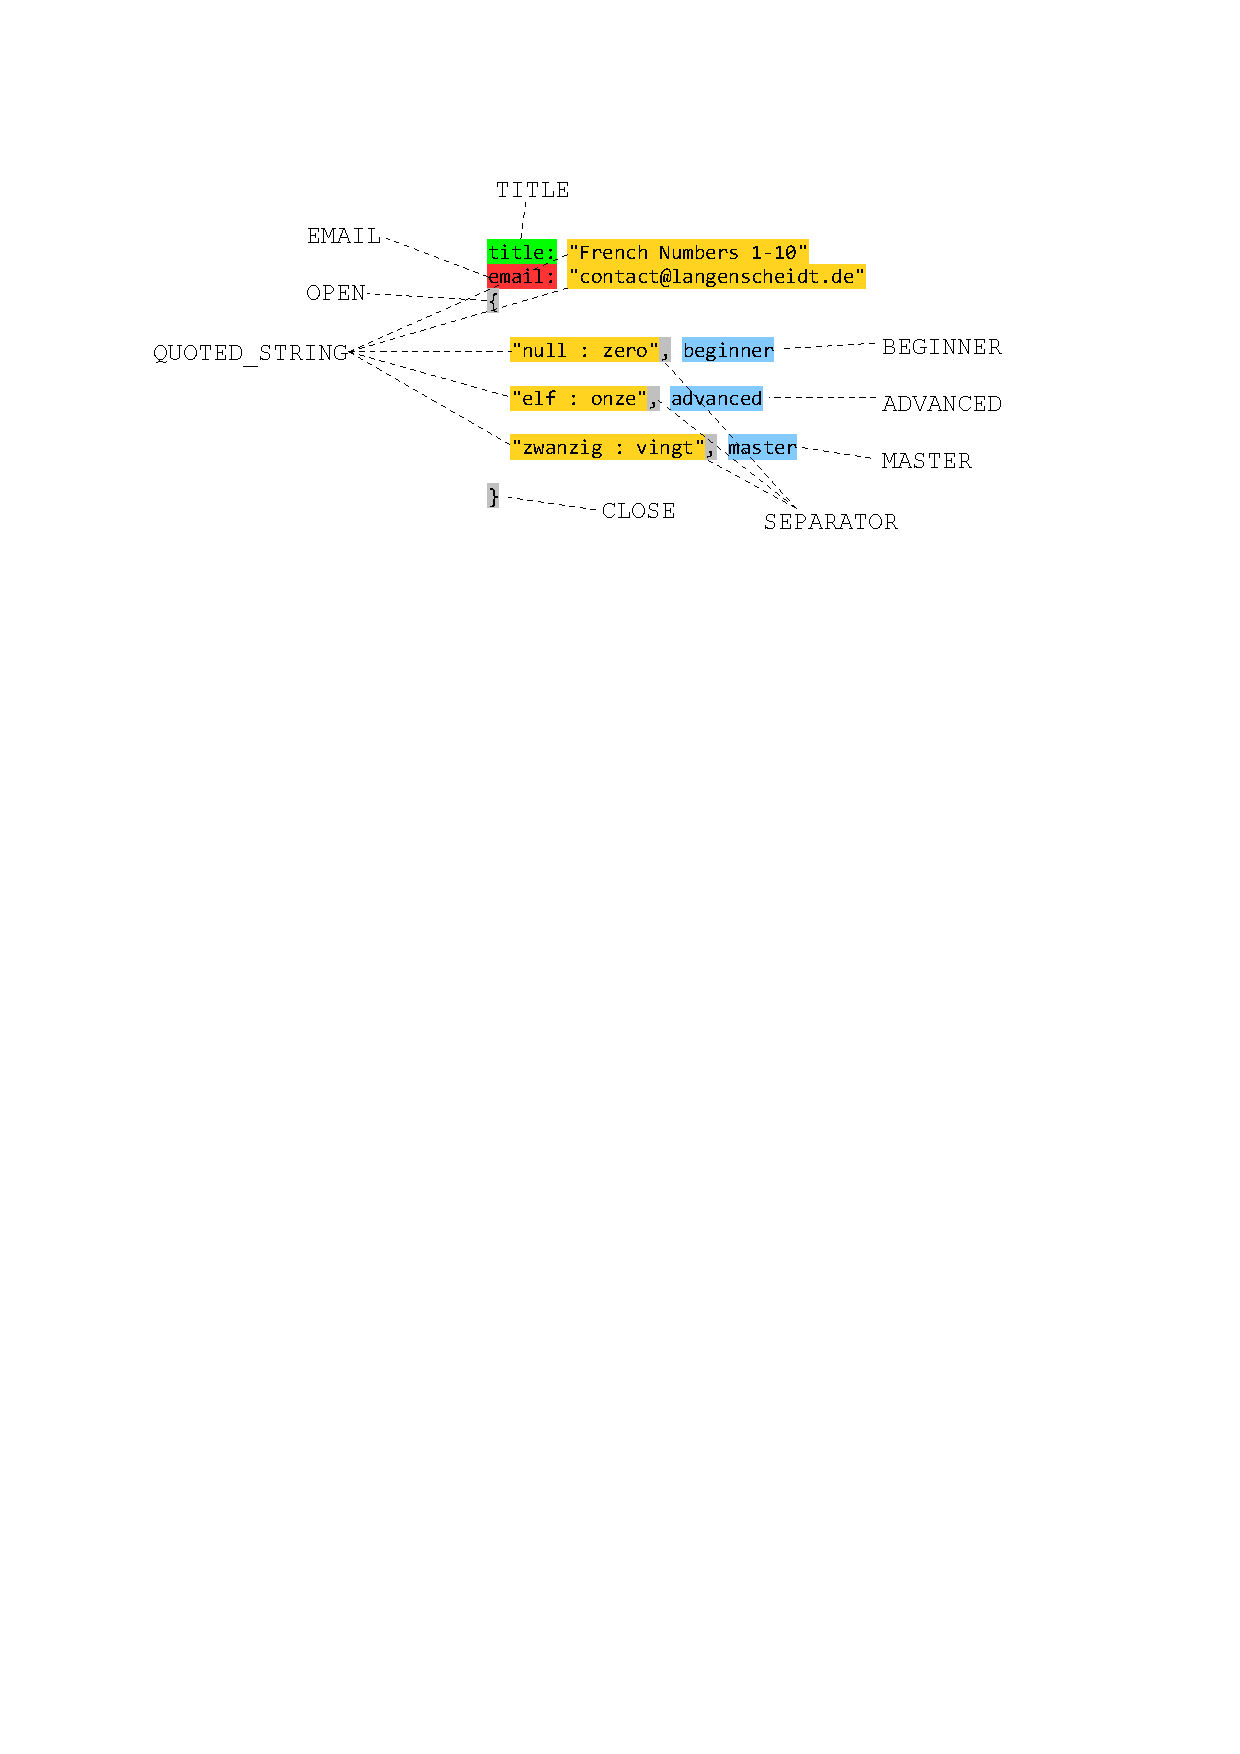
\includegraphics[width=0.8\textwidth]{4-tokens.pdf}
	\caption{Textual syntaf of a dictionary file} 
	\label{textual_syntax} 
\end{figure} 

\begin{itemize}
\item So open the \texttt{DictionaryLexer.g} file in \texttt{Dictionary\-Code\-Adap\-ter/\-src/\-org.\-moflon.\-moca.\-dictionary.\-parser} (Fig.~\ref{ParserFiles}).
\end{itemize}

\begin{figure}[htbp]
	\centering
	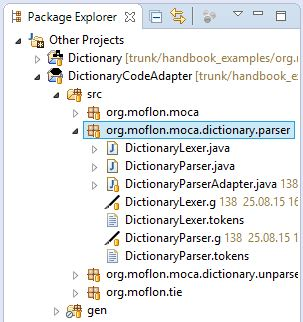
\includegraphics[width=0.5\textwidth]{eclipse_select_parser}
	\caption{Parser files} 
	\label{ParserFiles} 
\end{figure} 

As you can see in Fig.~\ref{DictionaryLexer} the tokens from Fig.~\ref{textual_syntax} has been specified.
\newline
Next we have to declare the parser grammar to complete the transformation.

\begin{figure}[htbp]
	\centering
	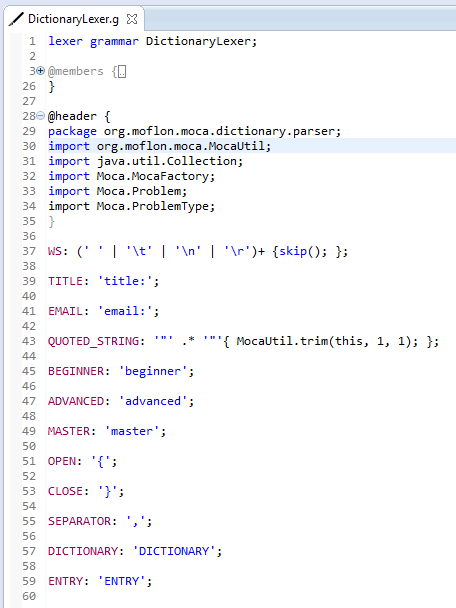
\includegraphics[width=0.7\textwidth]{eclipse_dictionaryLexer}
	\caption{DictionaryLexer.g file} 
	\label{DictionaryLexer} 
\end{figure} 

\begin{itemize}
\item For this open the DictionaryParser.g file (Fig.~\ref{ParserFiles}). 
\end{itemize}

You will quickly recognize that the parser grammar (Fig.~\ref{ParserGrammar}) is quite similar to the textual syntax from Fig.~\ref{textual_syntax}.

\begin{figure}[htbp]
	\centering
	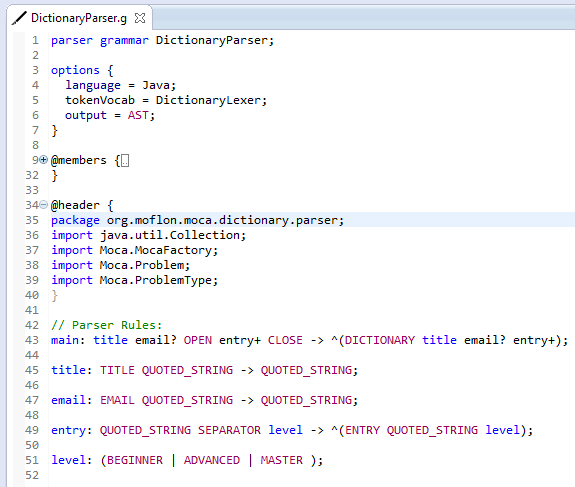
\includegraphics[width=0.9\textwidth]{eclipse_dictionaryParser}
	\caption{Parser grammar} 
	\label{ParserGrammar} 
\end{figure}

Now you have an overfiew of how to set up a parser in Moflon. But now lets see how this work. For this we transform some text files in an AST.

\begin{itemize}
\item We prepared some example files for you. So go to \texttt{instances/\-in/\-my\-Library/} (Fig.~\ref{ExampeFiles}) and have a look at the example files. They all have of course our above syntax.

\begin{figure}[htbp]
	\centering
	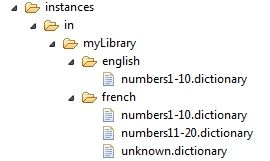
\includegraphics[width=0.55\textwidth]{inputData}
	\caption{Example files} 
	\label{ExampeFiles} 
\end{figure}

\item After you read through the example files, we have to run the transformation. Right click on \texttt{DictionaryCodeAdapterTrafo.java} in \texttt{Dic\-tionaryCodeAdapter/src/org.moflon.tie/} (Fig.~\ref{trafoExecution}) and navigate to \texttt{Run As/Java Application}. 

\begin{figure}[htbp]
	\centering
	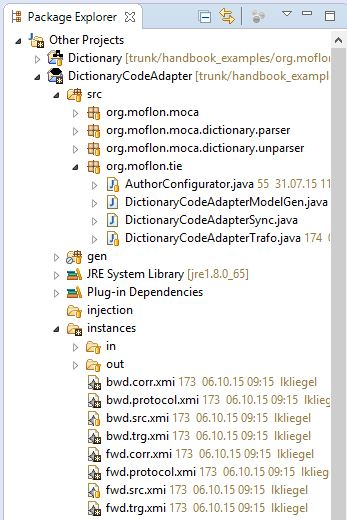
\includegraphics[width=0.6\textwidth]{transformationFiles}
	\caption{Transformation files} 
	\label{trafoExecution} 
\end{figure}

\item When the transformation is ready open in \texttt{instances} the \texttt{fwd.src.xmi} file to see the results of our transformation (Fig.~\ref{parserResults}).
\end{itemize}

\begin{figure}[htb]
	\centering
	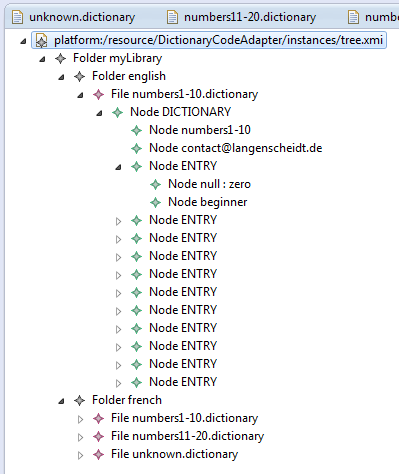
\includegraphics[width=0.75\textwidth]{eclipse_textParsingGeneration}
	\caption{Parser results} 
	\label{parserResults} 
\end{figure}

Here you can see that each language is transformed in an own folder and each file in an own subfolder with all its entries in it.
\newline
To get more information about the transformation and how to transform backword we recommend you to work through our handbook Part V.